\documentclass{report}
\title{CS246 Course Notes}
\usepackage{listings}
\usepackage{xcolor,color}
\usepackage{courier}
\usepackage{inconsolata}
%\renewcommand*\familydefault{\ttdefault}
\lstset{numbers=left,
numberstyle=\tiny,
keywordstyle=\color{blue!70}, commentstyle=,
frame=shadowbox,
rulesepcolor=\color{red!20!green!20!blue!20},
breaklines=true,
extendedchars=true
}


\definecolor{mykeycode}{RGB}{138,74,11}
\definecolor{mybg}{RGB}{64,64,64}
\definecolor{mycm}{RGB}{170,215,208}
\definecolor{mycode}{RGB}{219,219,219}


\lstset{language=C++,
numbers=left,
                basicstyle=\color{mycode}\ttfamily,
                keywordstyle=\color{mykeycode}\ttfamily,
                stringstyle=\color{red}\ttfamily,
                commentstyle=\color{mycm}\ttfamily,
                morecomment=[l][\color{magenta}]{\#},
                backgroundcolor=\color{mybg}, 
                morekeywords={*,string.cin}
}
\author{mzx!}
\date{\today}
\newcommand{\ibx}[1]{\framebox[1.1\width]{ #1 }}
\usepackage{amsmath,amssymb}
\usepackage{hyperref}
\usepackage{enumitem} 
\hypersetup{
    colorlinks,
    citecolor=black,
    filecolor=black,
    linkcolor=black,
    urlcolor=black
}

\PassOptionsToPackage{svgnames}{xcolor}
\usepackage{tcolorbox}
\usepackage{lipsum,xcolor,color}
\tcbuselibrary{skins,breakable}
\usetikzlibrary{shadings,shadows}

\definecolor{title_color}{HTML}{ea7dc7}
\definecolor{back_color}{HTML}{f7e8e8}

\newcounter{defboxctr}
\newenvironment{defbox}{%
\refstepcounter{defboxctr}% increment the environment's counter
    \tcolorbox[beamer,%
    noparskip,breakable,
    colback=back_color,colframe=title_color,%
    title={Definition \thedefboxctr}]}%
    {\endtcolorbox}
    \numberwithin{defboxctr}{section}





\begin{document}
\maketitle
\chapter{Midterm Structure}
\section{breakdown}
7-8 Questions in Total\\
\section{Definition Questions}
\begin{itemize}
\item[Q.1] Multiple Choice \\
Note that sometimes there are more than one correct choices
\item[Q.2] True or False
\item[Q.3] Short Answers
\end{itemize}
\section{Long Answer Questions}
\begin{itemize}
\item[Q.4] Bash Programming
\item[Q.5] Big 5 Programming
\item[Q.6] Big 5 Programming
\item[Q.7] Finding Error 
\end{itemize}
\section{NOT IN TEST}
Make File\\static
\chapter{Linux Shell Bash}
\section{Relative Path \& Absolute Path}
\paragraph{Absolute Path}
always starts with \ibx{/} or \ibx{$\sim$/}, and starts at root directory
\paragraph{Relative Path} starts from current directory,such as \ibx{bin/bash}

\section{Output Redirection \& Input Redirection}
\paragraph{Output Redirection} executes commands args and captures the output in the file instead of screen
\paragraph{Input Redirection} take the input from the file instead of the key board an display
\subsection{Shell Command About Directory}
\paragraph{For Relative Path} we use \ibx{.} as Current Directory (Relative),\ibx{..} as Parent Directory, \ibx{../..} as GrandParent (Relative),{\tiny Note that it is not "..."}.
\paragraph{For Absolute Path} we use \ibx{$\sim$} as Home Directory and \ibx{$\sim$userid} as User's Home Directory (Requires Permission)

\subsection{stdin/stdout/stderr}
\ibx{0} stdin, using \ibx{$<$} for input redirection\\\\
\ibx{1} stdout, using \ibx{$>$} for overwrite output redirection, using \ibx{$>>$} for append output redirection\\\\
\ibx{2} stderr
\section{Cat}
\begin{lstlisting}
cat input.txt // cat file
cat < input.txt // cat stdin
\end{lstlisting}
Both command gives same output

\section{Word Count}
Output format: \ibx{newline words bitscount}\\
\begin{lstlisting}
//in.txt: 
//this is it

wc in.txt // wc file
wc < input.txt //wc input
\end{lstlisting}
These two command gives \textbf{DIFFERENT} output, where "wc file" gives \ibx{1 3 3 in.txt} but "wc input" gives \ibx{1 3 3}. Note that the file name will not be produced with "wc input"

\section{Pattern Matching}
\subsection{WildCard Mathing/Globbing Matching}
\paragraph{WildCard Matching} uses \ibx{*} as "O or more any chars", \ibx{?} as single any char.
\begin{lstlisting}
*.cc // Any .cc files
test.* // Any file with name "test" no matter the extend

?.cc //all .cc file with a name in one char
\end{lstlisting}
\subsection{Regular Expression}
\paragraph{In Regular Expression} \ibx{.} represent \textbf{ANY SINGLE CHAR}.\ibx{+}: 1 or more preceding pattern. \ibx{*}: 0 or more preceding pattern. ibx{?}: 0 or 1 preceding pattern\\
Note that \ibx{*} in WildCard Matching = \ibx{.*} in Regular Expression\\
\ibx{$\wedge$} :Beginning of a line, 
\ibx{$\$$} : End of a line.\\
\ibx{(...|...|...)}: any one the given expressions\\
\ibx{[...]}: any character form this set \ibx{$[\wedge...]$} or \ibx{[!...]} any one of the characters not listed
\section{Quoting}
\ibx{\textbackslash}: Escapes any character\\
\ibx{``}: Open a shell and run what's in it in background\\
\ibx{''}: Don't allow variable to be expand, literally whatever is inside\\
\ibx{""}: Allow variable to expand, recognize escapes, back quotes,but DO NOT RUN COMMAND
\section{Pipe}
\paragraph{Pipes} use the output of one program as the input of another

\section{Testing}
\paragraph{Testing}cannot guarantee your program is correct, but can prove it's incorrect

\chapter{Shell Scripts}
\chapter{Inheritance}
\section{UML}
\subsection{OWNS-A / Composition}
when an object takes ownership if another object, Composition create an Owns-A relation. 
Embedding an object within another is composition\\
\ibx{A OWNS-A B}\\
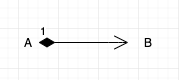
\includegraphics[width = 0.3\textwidth]{cs1}
\begin{itemize}
\item If A is copied, B is copied as well
\item If A is destroyed, B is destroyed
\end{itemize}
\paragraph{Examples} Basis OWNS-A Vector,Car OWNS-A Wheels
\begin{lstlisting}
class Car{
    Wheel w1,w2,w3,w4; 
    // With automatic delete w1,w2,w3,w4
    // If I want to destroy a car, its wheels get destroyed as well
    // If I want to copy a car, the duplicated car has wheels w1 w2 w3 w4 as well
}
\end{lstlisting}
\subsection{HAS-A / Aggregation}
\ibx{A HAS-A B}\\
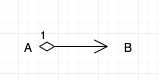
\includegraphics[width = 0.3\textwidth]{cs2}
\begin{itemize}
\item When A is copied, B is NOT
\item When A is destroyed, B is NOT
\item NOTE that someone else should take the ownership of B and delete B at some point
\end{itemize}
\paragraph{Examples}
Lake HAS-A Geese
\begin{lstlisting}
class Lake {
    Goose **geese;
};
    //If i want to delete the Lake, we are not gonna delete geese, but someone else should
    //We will delete the array, that contain the geese
\end{lstlisting}
\subsection{IS-A / Inheritance}
Inherites ALL(Public and Private) members(fileds as methods) from the Base Class\\
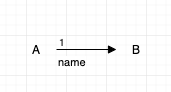
\includegraphics[width = 0.3\textwidth]{cs3}\\
\ibx{Book Collection}
\begin{itemize}
\item Text IS-A Book (with an extra topic field)
\item Comic IS-A Book (with an extra hero field)
\item Any method you can call on Book Object, you can call on a Text Object
\item Text inherits privates field, title, authors, numPages from BaseClass Book, they are not declared in Text class
\item Yet Text objects CANNOT access those fields
\item Yet we can not use MIL to construct a Text class
\end{itemize}

\end{document}
